\documentclass[a4paper]{article}

\usepackage{mathrsfs}
% ============================================
%         General Packages
% ============================================
\usepackage{balance}

\usepackage{kotex}      % for Korean
\usepackage{lipsum}     % for dummy text
\usepackage{array}

\usepackage{cite}   % for citation

\usepackage{amsmath,amsfonts}
\usepackage{amssymb}
\usepackage{soul}
\usepackage{mathrsfs}

\usepackage{hyperref}

    \hypersetup{
        pdftoolbar=false,        	% show Acrobat’s toolbar?
        pdfmenubar=false,        	% show Acrobat’s menu?
        pdffitwindow=false,     	% window fit to page when opened
        pdfstartview={FitH},    	% fits the width of the page to the window
        pdftitle={},    	% title
        pdfauthor={},     	% author
        %     pdfsubject={},   	% subject of the document
        %     pdfcreator={},   	% creator of the document
        %     pdfproducer={}, 	% producer of the document
        %     pdfkeywords={keyword1, key2, key3}, % list of keywords
        %     pdfnewwindow=true,      	% links in new PDF window
        colorlinks=true,       	% false: boxed links; true: colored links
        linkcolor=blue,          	% color of internal links (change box color with linkbordercolor)
        citecolor=blue,       	% color of links to bibliography
        filecolor=blue,      	% color of file links
        urlcolor=blue		% color of external links
    }

\usepackage{algorithm}
\usepackage{algorithmic}

\usepackage{epsfig}
\usepackage[dvipsnames]{xcolor}

% MY PACKAGES ===================================

\usepackage{svg}
\usepackage{subfig}

\usepackage{textcomp}
\usepackage{stfloats}
\usepackage{url}
\usepackage{verbatim}
\usepackage{graphicx}
\usepackage{multirow}
\usepackage{multicol}

\let\proof\relax
\let\endproof\relax
\usepackage{amsthm}
\usepackage{lipsum}
\usepackage{tikz}

% 
\usepackage{titlepic}
\usepackage{pdfpages}
\usepackage{etoolbox} % 조건문을 쓰기 위한 패키지


\titlepic{%
  
\includegraphics[height = 8mm]{figures/logo_KAIST_simple.png}
  \hspace{5mm}
  
\includegraphics[height = 8mm]{figures/MIC_Logo.png}
  }

% ========================================
%         TITLE and AUTHORS
% ========================================
\title{
  Structured Critic Adaptation
}

\author{
    Ahmad Mouri Zadeh Khaki
    \thanks{\href{https://kaist-mic-lab.github.io/members/aMouri/}{Ahmad Mouri Zadeh Khaki} is Postdoctoral Researcher at KAIST, {\tt\small ahmadmouri@kaist.ac.kr}}%
    , and 
    Jiyun Kim
    \thanks{\href{https://kaist-mic-lab.github.io/members/jyKim/}{Jiyun Kim} is Researcher at KAIST, {\tt\small JiyunKim@kaist.ac.kr}}%
}

\date{
    % 20\textsuperscript{th} March 2025
    Complied on \today
}

\begin{document}

\maketitle

% ========================================
%         Contents
% ========================================

\begin{figure}[h]
  \centering
  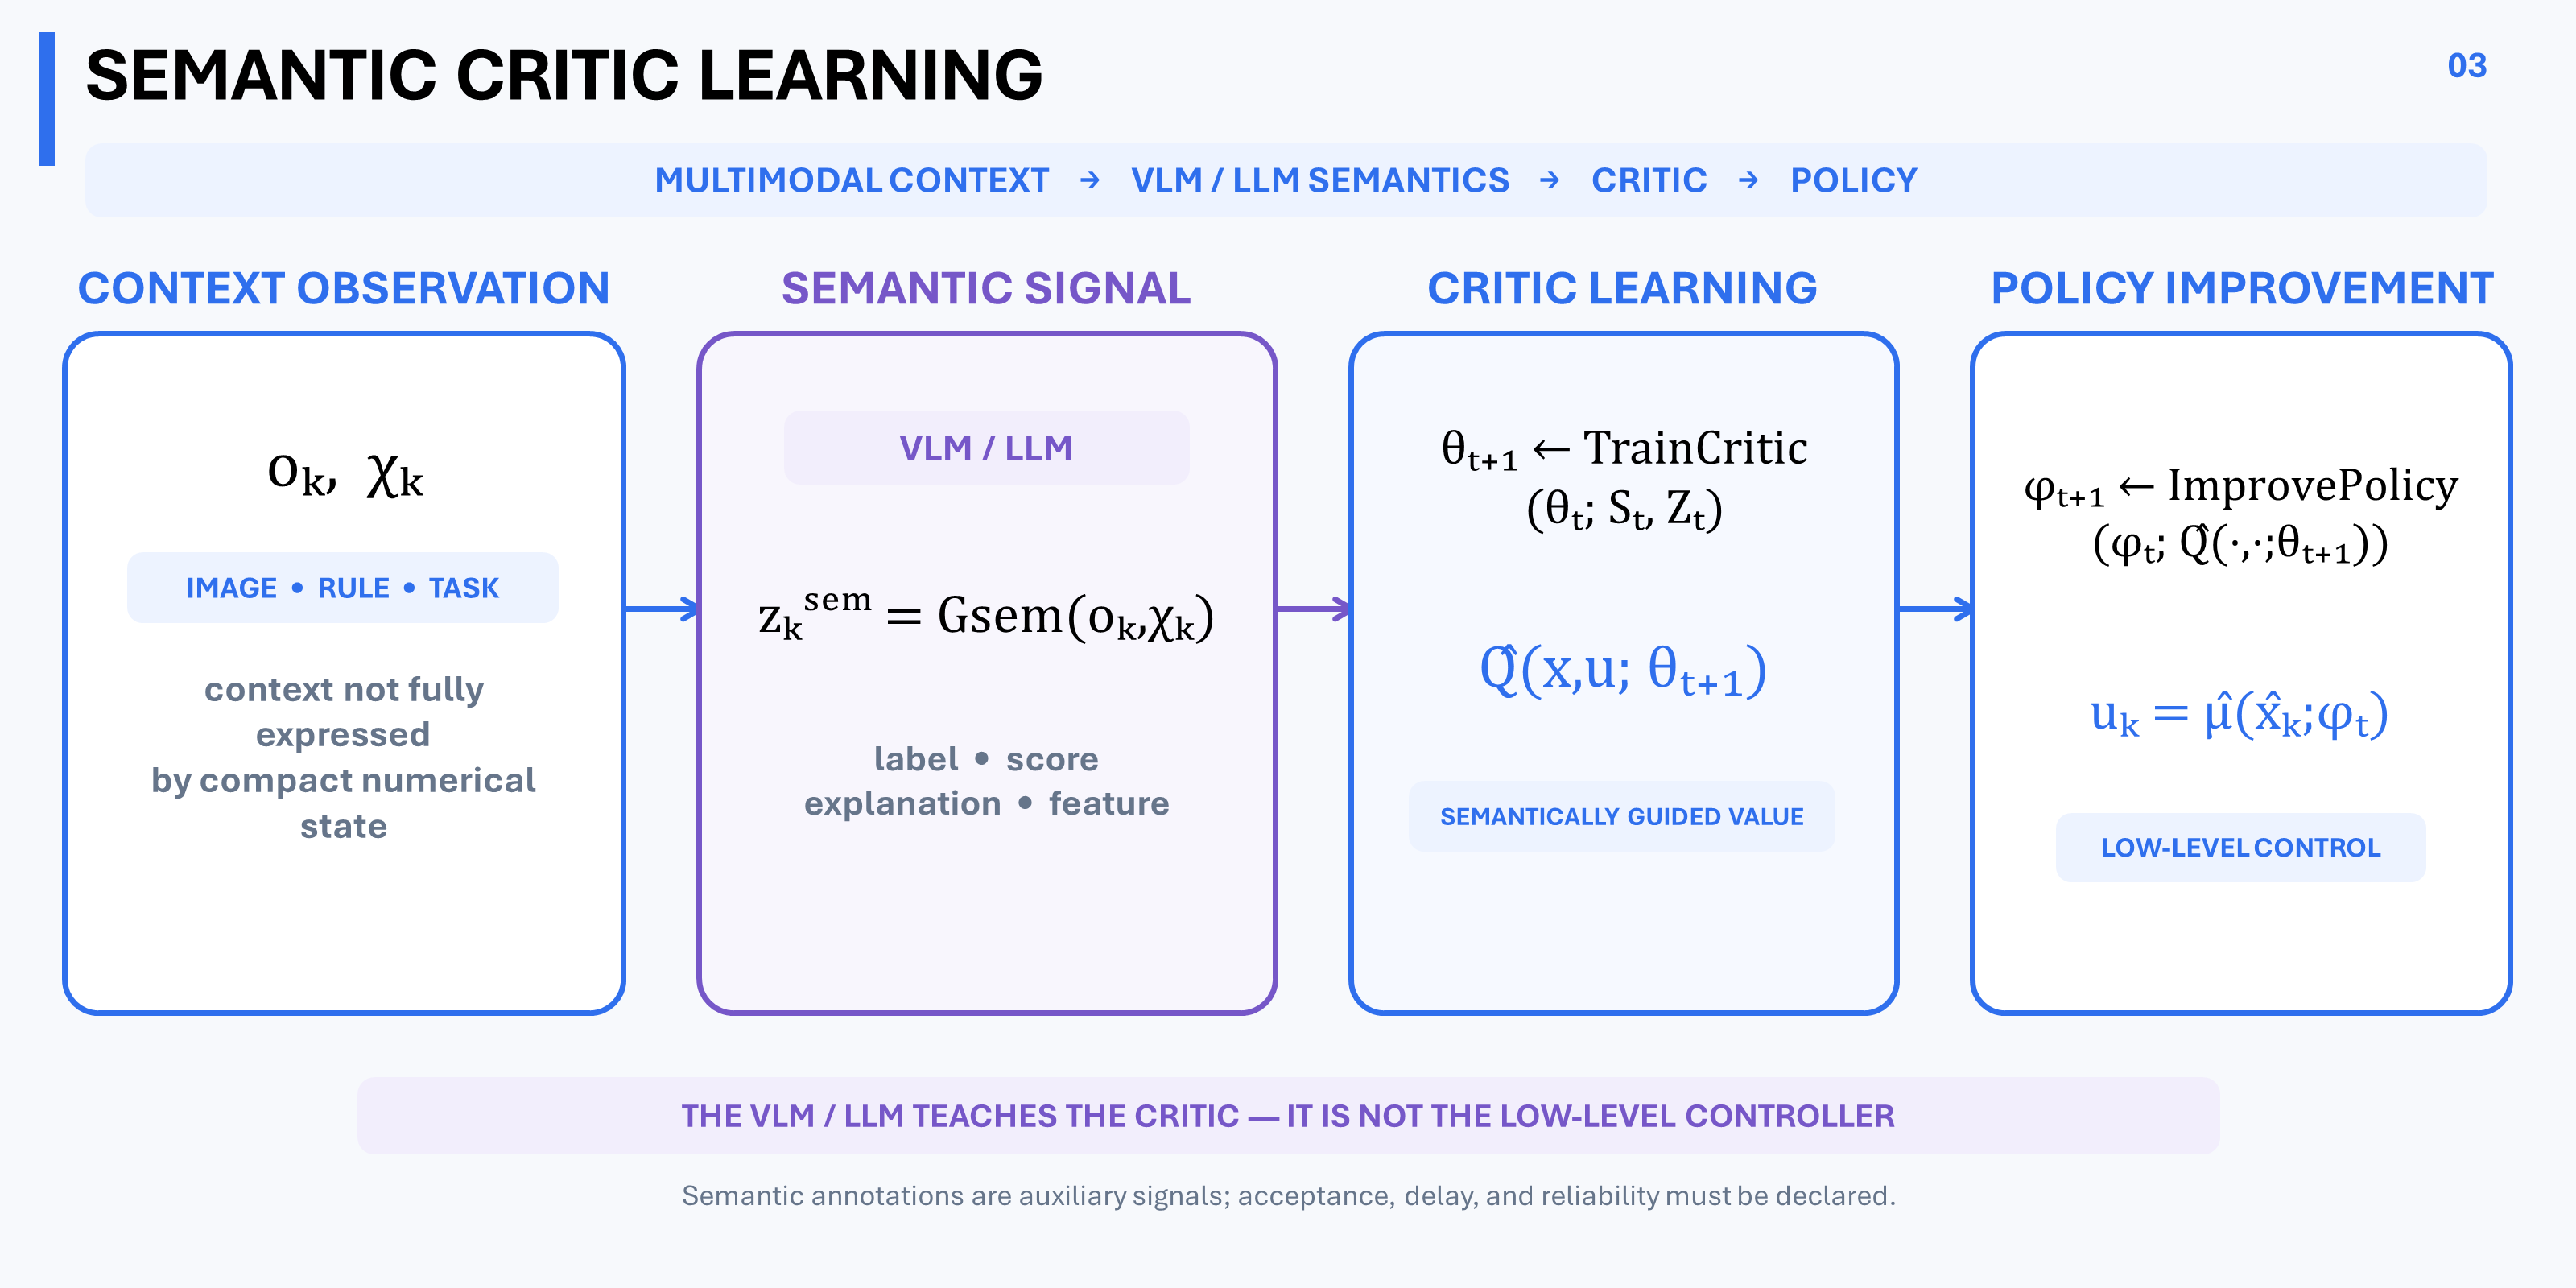
\includegraphics[width=\textwidth]{figures/03_semantic_critic_learning.png}
  \caption{Multimodal observations produce semantic annotations
    that provide auxiliary critic supervision alongside Bellman data, and the updated critic guides policy improvement.}
\label{fig:}
\end{figure}

Physical interaction is indexed by $k$, whereas critic and policy updates are
indexed by $t$. Semantic annotations may be generated offline,
asynchronously, or during operation; their timing and delay must be declared.
The figure shows the defining training-only route. Semantics required at
action time must instead enter the deployed information state.

\section{Problem definition}

\href{https://kaist-mic-lab.github.io/research/research_themes/RT_research_themes/}{Online Learning-Based Optimal Control}
defines a policy through a value or Q-function. Semantic Critic Learning
addresses cases in which multimodal or textual observations can provide
evaluation-relevant supervision not readily expressed by the standard
numerical transition and stage-cost record.

Let the controller receive a state estimate $\widehat x_k$, while $o_k$
contains observations such as images, scene relations, task descriptions, or
operator-provided rules. A VLM is suitable when visual and language context
must be interpreted together; an LLM can be used when the relevant context is
represented textually. Denote the selected high-level semantic interpreter by
$G_{\mathrm{sem}}$. It produces

\begin{equation}
z_k^{\mathrm{sem}}
=
G_{\mathrm{sem}}(o_k,\chi_k),
\end{equation}

where $\chi_k$ is optional task, prompt, or rule context.
$z_k^{\mathrm{sem}}$ is one semantic annotation, such as a label, score,
preference, explanation, or feature; it is not itself a control input. Before
entering a critic loss, a raw annotation must be mapped to a declared target,
comparison, constraint, or feature. In the notation below,
$G_{\mathrm{sem}}$ includes any required mapping and
$z_k^{\mathrm{sem}}$ denotes the resulting critic-usable annotation.

The defining case uses $z_k^{\mathrm{sem}}$ only as training supervision. If
semantic context is needed to distinguish deployed values or actions, it must
enter the controller-facing information state:

\begin{equation}
\xi_k=(\widehat x_k,z_k^{\mathrm{sem}}),\qquad
\widehat Q_\theta(\xi_k,u),\qquad
\widehat\mu_\phi(\xi_k).
\end{equation}

Here $z_k^{\mathrm{sem}}$ is a declared control-usable encoding available at
decision time, not unrestricted text. Training-only semantic targets must be
representable from the deployed information state; otherwise identical
deployed inputs can receive conflicting targets. Semantics that changes the
desired return requires an explicitly redefined stage cost and Bellman
object. It also does not by itself make a partially observed process Markov:
the controller still needs a sufficient observation history, belief state, or
learned information state.

Define a physical transition and the data selected at learning update $t$ as

\begin{equation}
d_k
=
(\widehat x_k,u_k,g_k,\widehat x_{k+1}),
\qquad
g_k
:=
g(\widehat x_k,u_k),
\qquad
\mathcal S_t
=
\{d_k:k\in\mathcal I_t\},
\end{equation}

where $\mathcal I_t$ is the set of physical transition indices selected for
update $t$. For an available annotation, let a predeclared rule decide whether
it is admitted:

\begin{equation}
a_k^{\mathrm{acc}}
:=
A_{\mathrm{sem}}
\!\left(
d_k,z_k^{\mathrm{sem}};\mathcal R_{\mathrm{acc}}
\right)
\in\{0,1\}.
\end{equation}

Set $a_k^{\mathrm{acc}}=0$ when no annotation is available, and define

\begin{equation}
\mathcal I_t^{\mathrm{sem}}
=
\left\{
k\in\mathcal I_t:
a_k^{\mathrm{acc}}=1
\right\}.
\end{equation}

Here $\mathcal R_{\mathrm{acc}}$ is the declared acceptance rule. It may check
schema and provenance, temporal assignment, consistency with measurements and
hard rules, and a calibrated confidence or agreement test. Raw VLM or LLM
self-confidence is not assumed to be calibrated. The gate
$a_k^{\mathrm{acc}}$ is determined before critic training; it is not optimized
with $\theta$.

The accepted paired dataset is

\begin{equation}
\mathcal Z_t
=
\left\{
(d_k,z_k^{\mathrm{sem}})
:
k\in\mathcal I_t^{\mathrm{sem}}
\right\}.
\end{equation}

Rejected or unavailable annotations do not remove $d_k$ from
$\mathcal S_t$; they only omit semantic supervision for that transition. For
compactness, the notation uses a common update batch. An asynchronous
implementation may reselect a retained transition when its annotation
arrives.

The learning path is represented conceptually as

\begin{equation}
\begin{aligned}
\theta_{t+1}
&\leftarrow
\operatorname{TrainCritic}
\!\left(
\theta_t;\mathcal S_t,\mathcal Z_t
\right),\\
\phi_{t+1}
&\leftarrow
\operatorname{ImprovePolicy}
\!\left(
\phi_t;\widehat Q_{\theta_{t+1}}
\right),
\end{aligned}
\end{equation}

where $\theta$ and $\phi$ are the critic and policy parameters. These
operators are conceptual rather than a commitment to one algorithm.
$\mathcal S_t$ supplies stage-cost and successor-state evidence for ordinary
Bellman or TD learning; $\mathcal Z_t$ supplies auxiliary semantic guidance
for the accepted subset.

The equations use a Q-factor because a sampled transition provides a direct
model-free critic target. A state-value critic $\widehat J_\theta$ can be used
instead when its successor-state and policy dependence are declared, as in
the overview figure.

\section{Why this problem matters}

A scalar stage cost provides one scalar evaluation channel, while images,
relations, or rules may support additional labels and comparisons: whether
another agent is yielding, whether a maneuver conflicts with a contextual
rule, or whether two outcomes should be evaluated differently.

A VLM or LLM may provide such high-level context as an auxiliary learning
signal without being placed directly in the fast control loop. The research
question is whether Bellman-compatible semantic supervision can improve
task-level evaluation by the critic and, through that critic, improve the
policy. Because the semantic model is fallible and distribution-dependent,
richer context is not by itself evidence of safety, optimality, or
generalization.

\section{Key challenges}

\begin{itemize}
  \item \textbf{Physical grounding and semantic reliability:} a semantic annotation can
  conflict with measurements, dynamics, action feasibility, or operating
  constraints. Designing and calibrating the acceptance rule, rejection
  behavior, and fallback path is therefore part of the method.
  \item \textbf{Closed-loop timing and causal attribution:} semantic annotations may be
  delayed, asynchronous, or stale. They must be assigned to the state--action
  transitions that caused the evaluated outcome without future-data leakage.
  \item \textbf{Control-objective and safety consistency:} semantic supervision may
  change which decisions the critic prefers. Its role in the objective or
  information state must be declared, and closed-loop evidence must separate
  its effect from extra data, reward tuning, or imitation while evaluating
  performance and constraint violations.
\end{itemize}

\section{Established approaches --- semantic rewards and policy guidance}

\textbf{Semantic reward specification or shaping.} An LLM can act as a proxy reward
function, while a VLM can score visual observations against a language-defined
goal (\href{https://openreview.net/forum?id=10uNUgI5Kl}{Kwon et al., 2023};
\href{https://proceedings.iclr.cc/paper_files/paper/2024/hash/7a7f6cc5dc2a84fb4edf0feb8e5cfd50-Abstract-Conference.html}{Rocamonde et al., 2024}).
The resulting semantic score modifies the cost used by an otherwise standard
RL algorithm:

\begin{equation}
\widetilde g_k
=
g_k+\lambda_{\mathrm{rew}}s_k^{\mathrm{sem}},
\qquad
\lambda_{\mathrm{rew}}\ge0,
\end{equation}

so the critic and policy optimize the modified return. This is a reward-level
route, and an arbitrary semantic term can change the control objective. Here
$s_k^{\mathrm{sem}}$ is defined as a semantic \textbf{cost} or penalty, so a larger
value is less desirable; if a semantic model produces a reward-like score,
its sign must be converted before it is added to the cost.

\textbf{Preference-derived reward learning.} Instead of requesting a raw scalar
score, human or VLM feedback can compare trajectory segments or observations.
A separate reward model is then learned from those preferences and supplied
to RL (\href{https://papers.nips.cc/paper/7017-deep-reinforcement-learning}{Christiano et al., 2017};
\href{https://proceedings.mlr.press/v235/wang24bn.html}{Wang et al., 2024}).
Semantics still reaches the critic through a scalar learned reward.

\textbf{Direct policy guidance.} A preferred semantic action or demonstration can
supervise the policy without defining a critic-level learning signal:

\begin{equation}
\mathcal L_{\mathrm{IL}}(\phi)
=
-
\sum_{k\in\mathcal I_{\mathrm{IL}}}
\log
\pi_\phi
\!\left(
u_k^{\mathrm{sem}}\mid\widehat x_k
\right).
\end{equation}

$\mathcal I_{\mathrm{IL}}$ indexes semantic demonstrations, and
$u_k^{\mathrm{sem}}$ is the preferred or demonstrated action.
Language-conditioned imitation is an established example of this direct route
(\href{https://www.roboticsproceedings.org/rss17/p047.html}{Lynch and Sermanet, 2021}).
The stochastic-policy symbol $\pi_\phi$ is used here because the displayed
loss is a likelihood-based imitation objective; the default control-policy
symbol elsewhere in these pages remains $\mu_\phi$.

\section{Research direction --- critic-level semantic supervision}

The proposed direction keeps physical transitions and stage costs in an
explicit Bellman loss while adding a separate semantic supervision term. The
equations below use the training-only case defined in Section 1, with deployed
critic and policy inputs $\widehat x$.

For a nonempty update set $\mathcal S_t$ and a declared nonnegative TD-residual
loss $\ell_{\mathrm{TD}}$, write

\begin{equation}
\begin{aligned}
\mathcal L_{\mathrm{Bellman}}
\!\left(
\theta;\mathcal S_t
\right)
&=
\frac{1}{|\mathcal S_t|}
\sum_{k\in\mathcal I_t}
\ell_{\mathrm{TD}}
\!\left(
\widehat Q_\theta(\widehat x_k,u_k)
-
y_{k,t}^{\mathrm{TD}}
\right),\\
y_{k,t}^{\mathrm{TD}}
&=
g_k
+
\alpha
\widehat Q_{\bar\theta_t}
\!\left(
\widehat x_{k+1},
\widehat\mu_{\bar\phi_t}(\widehat x_{k+1})
\right),
\end{aligned}
\end{equation}

where $(\bar\theta_t,\bar\phi_t)$ are fixed target parameters during update
$t$, and $0<\alpha<1$ is the discount factor. This is an approximate one-step
policy-evaluation target associated with the target policy
$\widehat\mu_{\bar\phi_t}$, not an optimal-Q target. Using data generated by
another behavior policy requires the usual coverage or off-policy assumptions.

The accepted annotations provide a separate critic-level supervision term:

\begin{equation}
\theta_{t+1}
\approx
\arg\min_\theta
\left\{
\mathcal L_{\mathrm{Bellman}}(\theta;\mathcal S_t)
+
\lambda_{\mathrm{sem},t}
\mathcal L_{\mathrm{sem}}(\theta;\mathcal Z_t)
\right\},
\qquad
\lambda_{\mathrm{sem},t}\ge0,
\end{equation}

\begin{equation}
\mathcal L_{\mathrm{sem}}(\theta;\mathcal Z_t)
=
\begin{cases}
\displaystyle
\frac{1}{|\mathcal Z_t|}
\sum_{(d_k,z_k^{\mathrm{sem}})\in\mathcal Z_t}
\ell_{\mathrm{sem}}
\!\left(
\widehat Q_\theta;
d_k,z_k^{\mathrm{sem}}
\right),
& |\mathcal Z_t|>0,\\
0,
& \text{otherwise},
\end{cases}.
\end{equation}

The acceptance rule has already removed rejected annotations, so this
overview weights the accepted pairs equally. A later implementation may use
separately calibrated confidence weights, but their source and calibration
must be declared; raw VLM or LLM self-confidence is not treated as a
probability of correctness.

$\lambda_{\mathrm{sem},t}$ controls the relative contribution of semantic
supervision. To retain $\widehat Q_\theta$ as a critic for the original stage
cost $g$, $\ell_{\mathrm{sem}}$ is limited to accepted value comparisons or
terminal labels that are demonstrably compatible with that return. A
comparison may reference another transition or trajectory segment through
$z_k^{\mathrm{sem}}$. A new preference or risk specification instead requires
an explicitly redefined objective or constraint; conflicting labels that
reveal missing decision context require an augmented deployed information
state.

The updated critic then guides policy improvement:

\begin{equation}
\phi_{t+1}
\leftarrow
\operatorname{ImprovePolicy}
\!\left(
\phi_t;\widehat Q_{\theta_{t+1}}
\right).
\end{equation}

A deployable method also needs annotation provenance, delay and cache
handling, rejection, and fallback rules.

Evaluation should compare a nonsemantic critic, numerical reward shaping,
semantic reward or reward-model baselines, direct semantic imitation, and the
critic-level formulation above. Relevant metrics include Bellman error,
critic calibration, control performance, semantic acceptance and rejection,
constraint violations, inference and update time, annotation sensitivity,
and contextual distribution shift.

\section{Application domains}

\begin{itemize}
  \item \textbf{Autonomous-driving decision and motion planning}, where visual scene
  relations, road conventions, and interaction context may provide auxiliary
  critic supervision or, when available online, augment the decision state.
  \item \textbf{Human--robot and language-conditioned control}, where task semantics
  may supervise value evaluation without unrestricted language output driving
  actuators.
  \item \textbf{Mobility and energy-management systems with contextual operating rules},
  including exceptional modes difficult to encode in one handcrafted scalar
  cost.
\end{itemize}

\section{References}

\begin{itemize}
  \item M. Kwon, S. M. Xie, K. Bullard, and D. Sadigh, ``Reward Design with
  Language Models,'' \textit{International Conference on Learning
  Representations (ICLR)}, 2023.
  \href{https://openreview.net/forum?id=10uNUgI5Kl}{Paper}
  \item J. Rocamonde, V. Montesinos, E. Nava, E. Perez, and D. Lindner,
  ``Vision-Language Models are Zero-Shot Reward Models for Reinforcement
  Learning,'' \textit{ICLR}, 2024.
  \href{https://proceedings.iclr.cc/paper_files/paper/2024/hash/7a7f6cc5dc2a84fb4edf0feb8e5cfd50-Abstract-Conference.html}{Paper}
  \item P. F. Christiano et al., ``Deep Reinforcement Learning from Human
  Preferences,'' \textit{Advances in Neural Information Processing Systems}, vol. 30,
  2017.
  \href{https://papers.nips.cc/paper/7017-deep-reinforcement-learning}{Paper}
  \item Y. Wang et al., ``RL-VLM-F: Reinforcement Learning from Vision Language
  Foundation Model Feedback,'' \textit{Proceedings of the 41st International
  Conference on Machine Learning}, PMLR 235, pp. 51484--51501, 2024.
  \href{https://proceedings.mlr.press/v235/wang24bn.html}{Paper}
  \item C. Lynch and P. Sermanet, ``Language Conditioned Imitation Learning Over
  Unstructured Data,'' \textit{Robotics: Science and Systems XVII}, 2021.
  \href{https://www.roboticsproceedings.org/rss17/p047.html}{Paper}
\end{itemize}

\end{document}
